
\documentclass{beamer}
\usetheme{Zurich}
\usepackage{amsmath, amsfonts, graphicx, multirow}
\title{Classifying the supernova data}
\author{Charlotte Wickham}
\date{\today}

\begin{document}

\frame{\titlepage}

\section[Outline]{ 	}
\frame{\tableofcontents}

\AtBeginSection[]
{
   \begin{frame}
       \frametitle{Outline}
       \tableofcontents[currentsection]
   \end{frame}
}


\begin{frame}
	\frametitle{Supernova data}
	\begin{itemize}
		\item Collection of 5000 supernova and 5000 other objects
		\item 19 features transformed by Raquel
		\item Split into balanced training and test sets.  9000 in training set, 1000 in test set.
	\end{itemize}
\end{frame}

\begin{frame}
	\frametitle{Summary}
	Error rates:
\begin{enumerate}

	\item 	Support vector machines $\approx$ 5\%

	\item 	Neural Networks $\approx$ 5\%

	\item 	Random Forests $\approx$ 5\%

	\item 	Bagged Trees $\approx$ 6\%

	\item 	Classification Trees $\approx$ 8\%

	\item 	Boosted Trees $\approx$ 9\%

\end{enumerate}

\end{frame}


\section{Support vector machines}

\begin{frame}
	\frametitle{Training svm}
	\begin{itemize}
				\item Kernel Function
				
				Radial basis function kernel
				\[
				\exp(-\gamma |u-v|^2)
				\]
				\item 10 fold cross validation to search for good parameters
				\item Parameters in kernel function

				$\gamma$:  14 values between 0.0001 and 5
				
				\item Tuning parameter (how much misclassification are we allowing?)
				
				search over 10 values between 0.5 and 100
	\end{itemize}
\end{frame}


\begin{frame}
	
	\frametitle{Best Support Vector Machine}
	$\gamma = 0.05 $ cost = 9
	\begin{table}
	\begin{tabular}{cr|rr}
	& & \multicolumn{2}{c}{Prediction}\\
	& & Other & Supernova\\
	\hline
	\multirow{2}{*}{\rotatebox{90}{Actual}} & Other &  484 &  16\\
	& Supernova & 32 &  468\\
	\end{tabular}
	\end{table}
	Error = 4.8\%

\end{frame}

\section{Trees}
	\begin{frame}
		\frametitle{Classification Trees}
		\begin{itemize}
			\item Grow full size tree - will tend to over fit
			\item Prune back using cross validation
		\end{itemize}
	\end{frame}

	\begin{frame}
	\frametitle{Pruned tree -  has 14 splits}
	\setkeys{Gin}{width=\textwidth}
	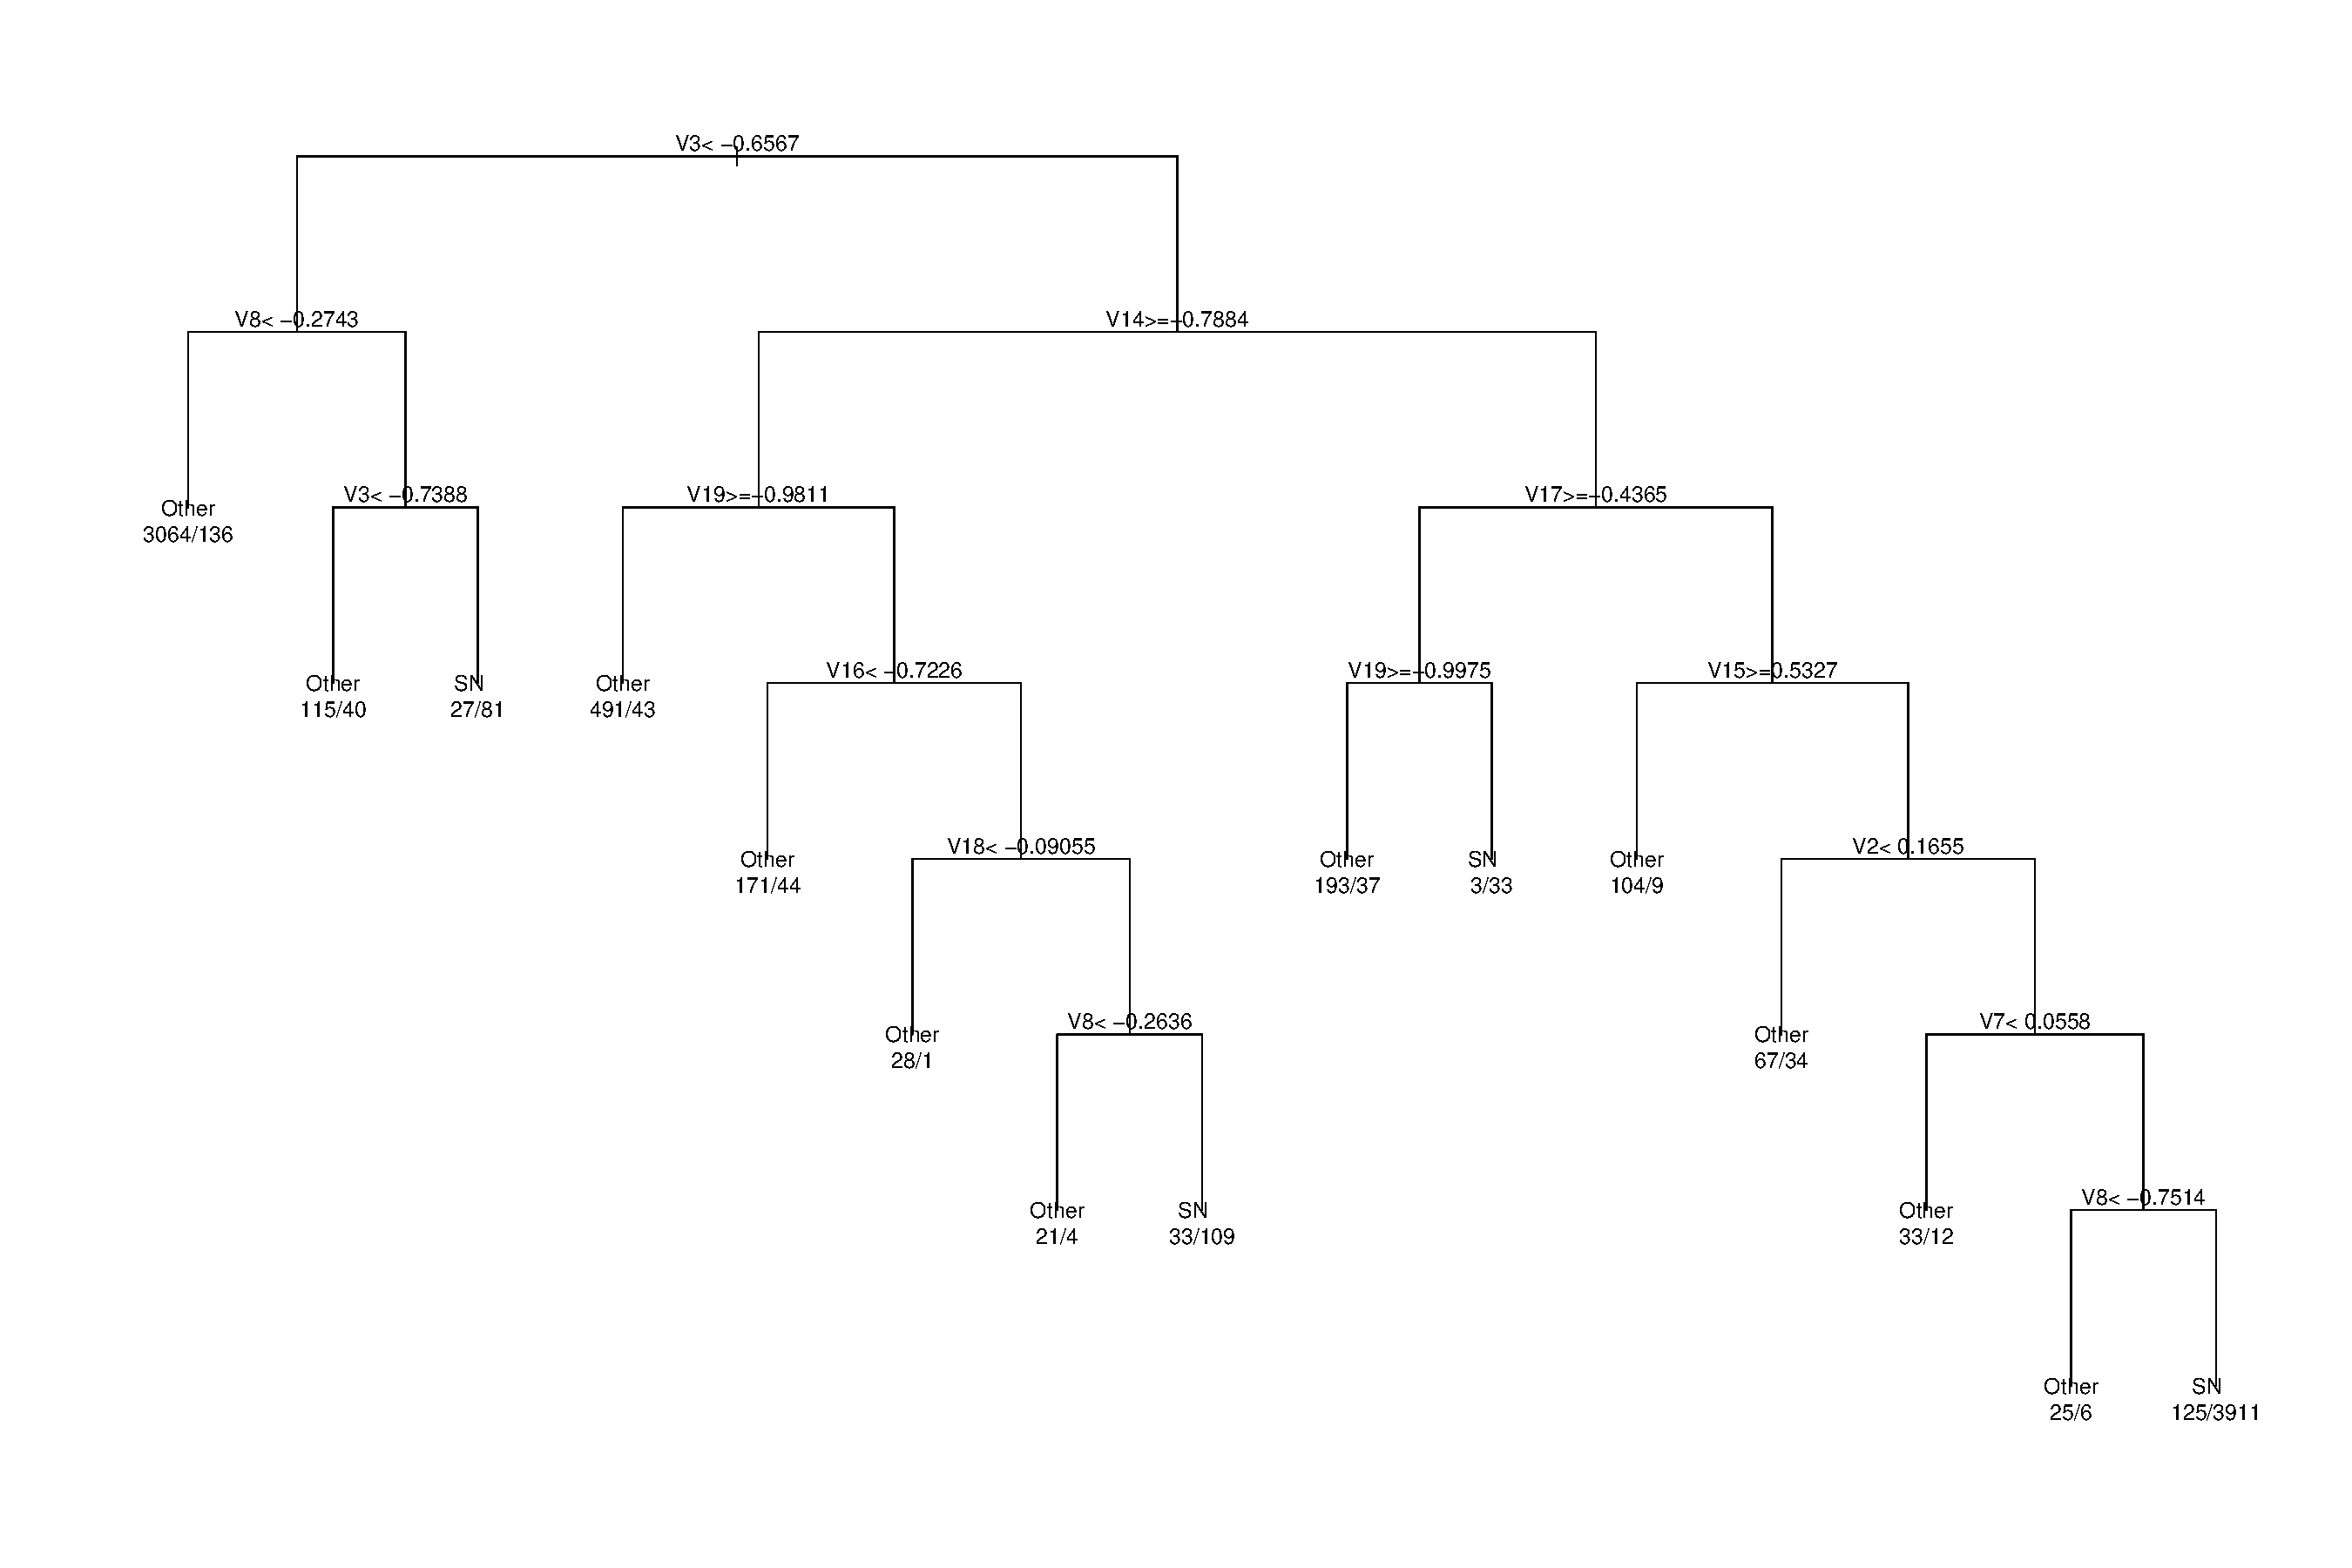
\includegraphics{tree.pdf}
	\end{frame}

	\begin{frame}
	\frametitle{Left branch}
	\begin{columns}[c] 
		\column{.6\textwidth} 
			\setkeys{Gin}{width=\textwidth}
			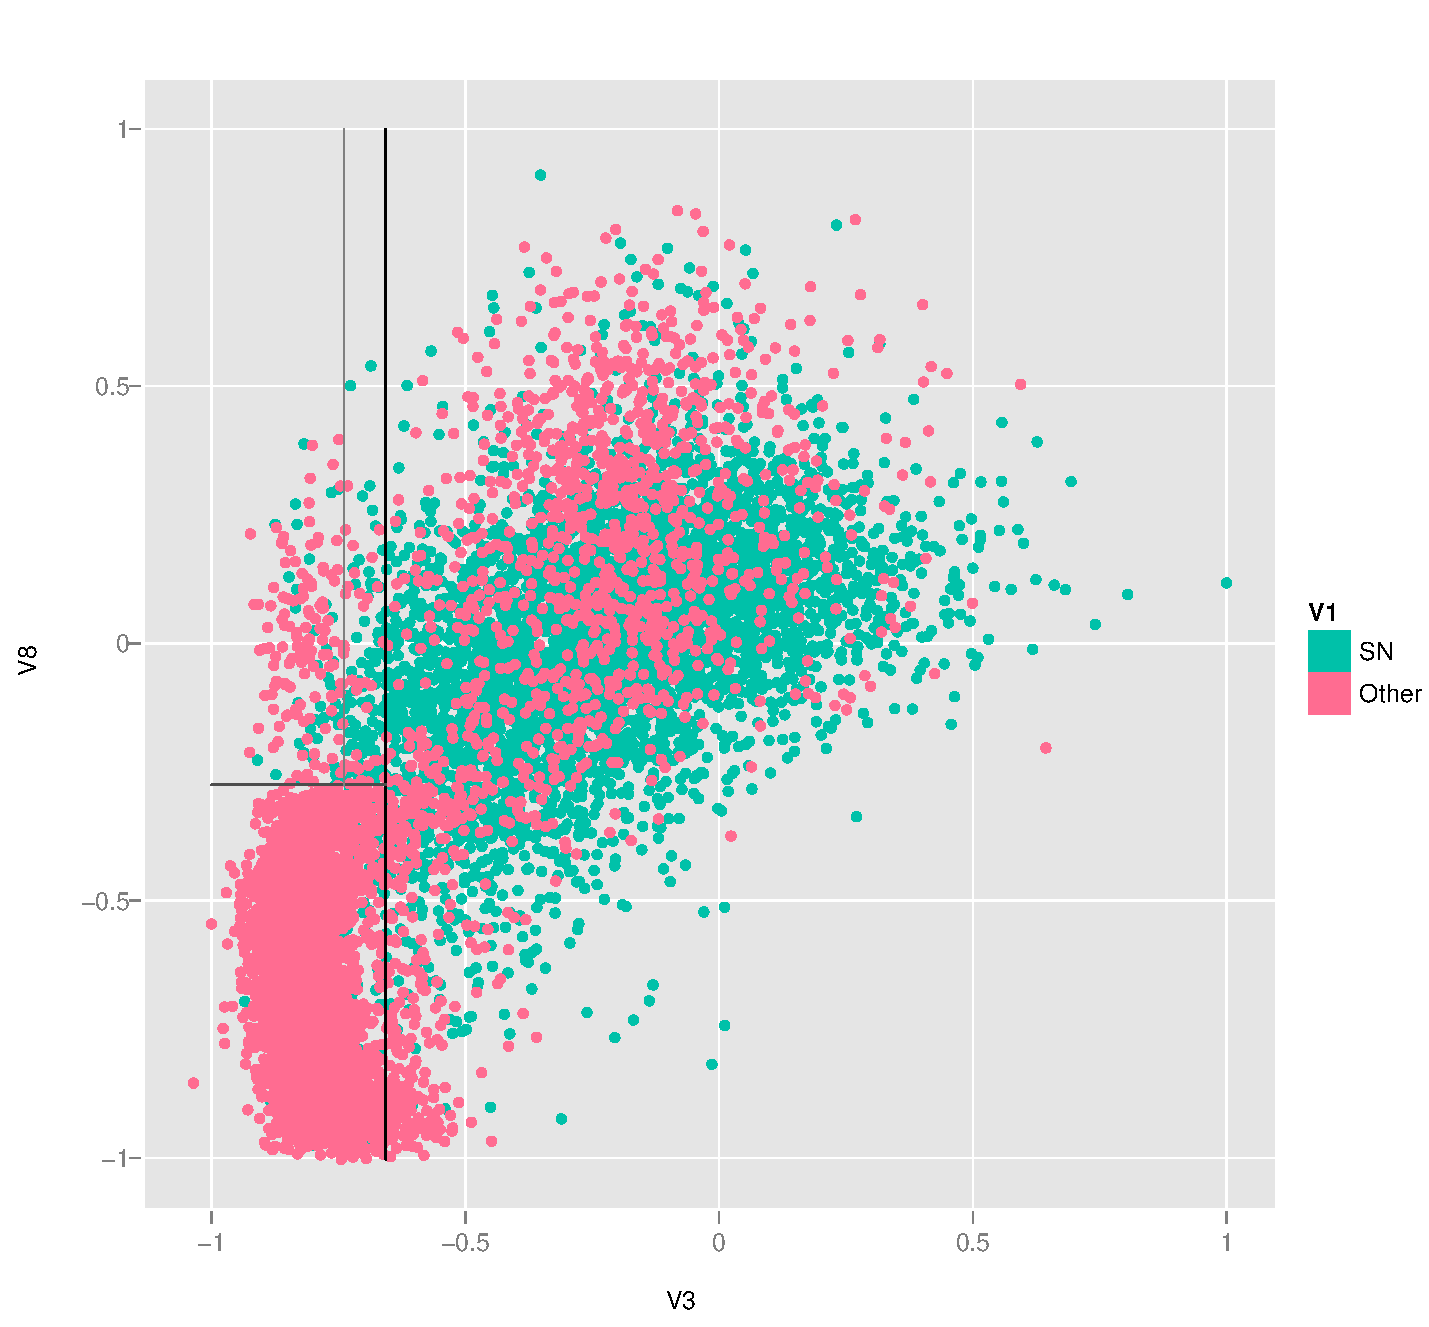
\includegraphics{leftside.pdf}
		\column{.4\textwidth}
			Splits on two variables classified a lot of the ``Other'' objects.
			They were:
			\begin{itemize}
				\item perinc (V3) - \% flux increase in aperture from REF to NEW 
			 	\item neighbordist (V8) - distance to the nearest object in REF 
			\end{itemize}		
	\end{columns}
	
	\end{frame}

	\begin{frame}
		\frametitle{Performance on test set}
		\begin{itemize}
			\item{Classification Tree
			\begin{table}
			\begin{tabular}{cr|rr}
			& & \multicolumn{2}{c}{Prediction}\\
			& & Other & Supernova\\
			\hline
			\multirow{2}{*}{\rotatebox{90}{Actual}} & Other &  461 &  39\\
			& Supernova & 45 &  455\\
			\end{tabular}
			\end{table}
			Error = 8.4\%}
		\end{itemize}
\end{frame}


\begin{frame}
	\frametitle{Adding costs and priors}
	\begin{itemize}
		\item See a lot more other objects than supernova
		\item Would like to be more accurate identifying non supernova to minimize false discoveries.
		\item Trees have the option of accounting for this by adding priors or misclassification costs.
		\item Priors didn't work too well
	\end{itemize}
\end{frame}


\begin{frame}
	\frametitle{Costs in supernova data}
	Costs: $C(SN|Other)=2, C(Other|SN)=1$
	\begin{columns}[c] 
		\column{.6\textwidth} 
			\setkeys{Gin}{width=\textwidth}
			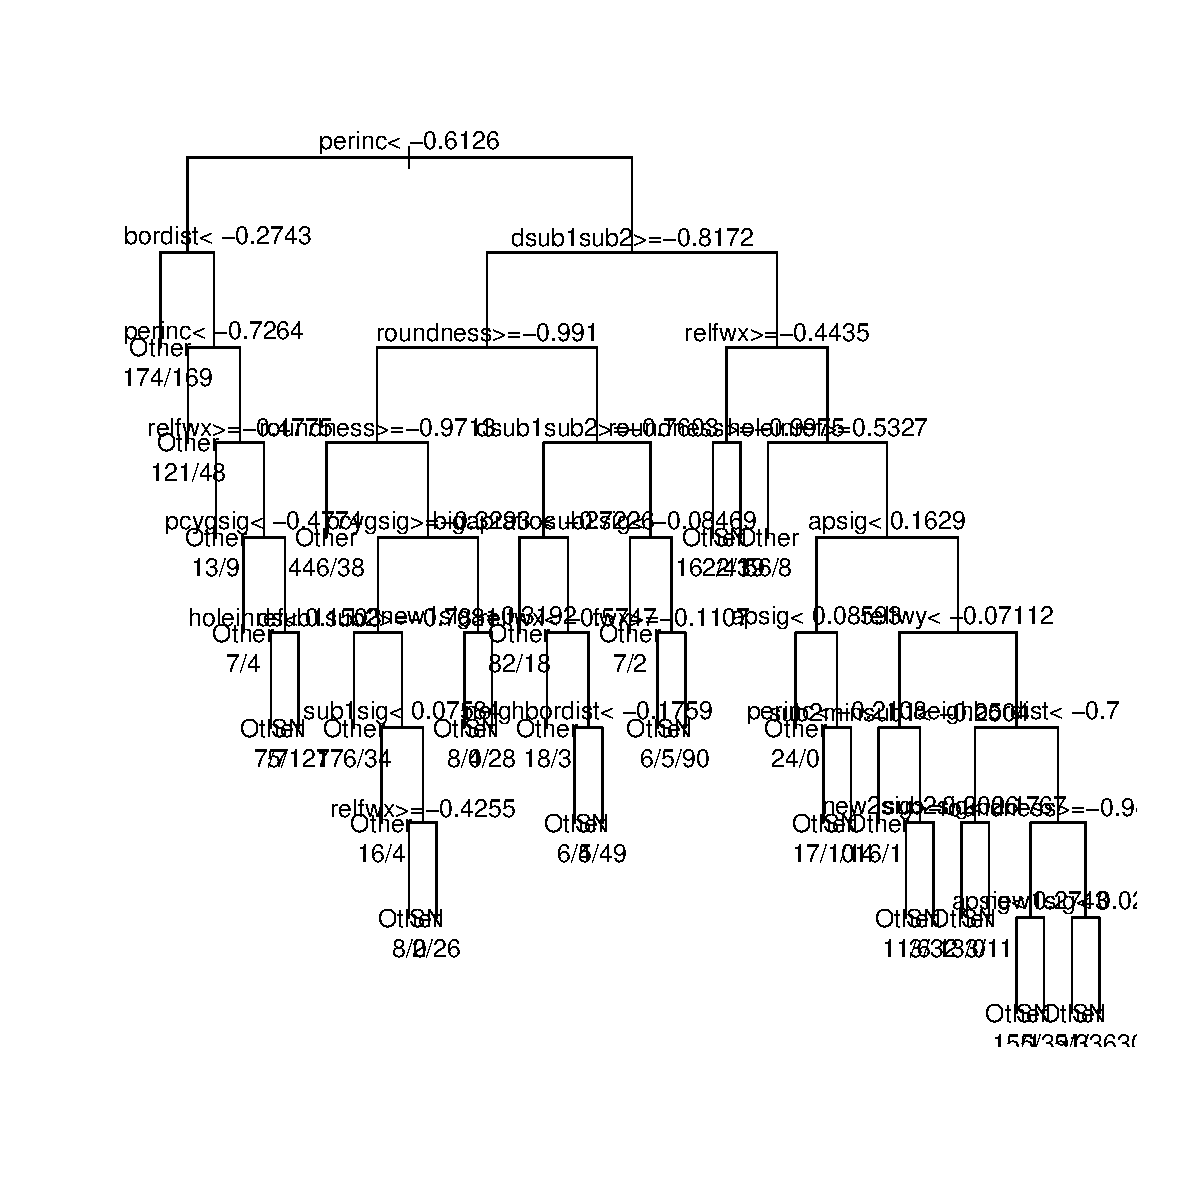
\includegraphics{treec1.pdf}
		\column{.4\textwidth}
				\begin{table}
				\begin{tabular}{cr|rr}
				& & \multicolumn{2}{c}{Prediction}\\
				& & Other & SN\\
				\hline
				\multirow{2}{*}{\rotatebox{90}{Actual}} & Other &  476 &  24\\
				& SN & 55 &  445\\
				\end{tabular}
				\end{table}	
				Total error = 7.9\%
				
				+ve's = 11\%
				
				-ve's = 4.8\%
			\end{columns}
\end{frame}


\section{Bagging}

\begin{frame}
	\frametitle{Bagging for trees}
	\begin{enumerate}
		\item A bootstrap sample, $\mathcal{L}_B$, from $\mathcal{L}$ is selected.
		\item A tree is grown on $\mathcal{L}_B$ (and $\mathcal{L}$ is used to choose a pruned subtree).
		\item This is repeated $K$ times to give a sequence of predictors, $\phi_1(x), \ldots, \phi_K(x)$.
		\item The bagged predictor of, $y_n$, is  $\text{avg}_k \phi_k(x_n)$ for regression trees or is the class having the plurality  in  $\phi_1(x), \ldots, \phi_K(x)$ for classification trees.
	\end{enumerate}
	Note: Bagging isn't restricted to trees.
\end{frame}

\begin{frame}
	\frametitle{Bagging Supernova data}
	\begin{table}
	\begin{tabular}{cr|rr}
	& & \multicolumn{2}{c}{Prediction}\\
	& & Other & SN\\
	\hline
	\multirow{2}{*}{\rotatebox{90}{Actual}} & Other &  477 &  37\\
	& SN & 23 &  463\\
	\end{tabular}
	\end{table}
		Total error = 6\%
		
		+ve's = 11.6\%
		
		-ve's = 4.6\%
\end{frame}

\section{Random forests}

\begin{frame}[fragile]
	\frametitle{Random input selection}
	Fix parameter $K$
	\begin{itemize}
		\item Draw a bootstrap sample from the training set
		\item Grow full size tree as usual except at each node choose $K$ variables randomly on which to search for the best split.
		\item Repeat $N$ times to generate $N$ trees.
	\end{itemize}
	Breiman suggests $K=\sqrt{\text{number of variables}}$.
	
\end{frame}

\begin{frame}
	\frametitle{Performance on test set}
	K = 4
	\begin{table}
	\begin{tabular}{cr|rr}
	& & \multicolumn{2}{c}{Prediction}\\
	& & Other & Supernova\\
	\hline
	\multirow{2}{*}{\rotatebox{90}{Actual}} & Other &  484 &  16\\
	& Supernova & 39 &  461\\
	\end{tabular}
	\end{table}
	Error: 5.5\%
	
	(were getting about 8\% from CART and 6\% from bagging.)
\end{frame}

\begin{frame}
	\frametitle{Supernova - Variable Importance}
	\setkeys{Gin}{width = \textwidth}
	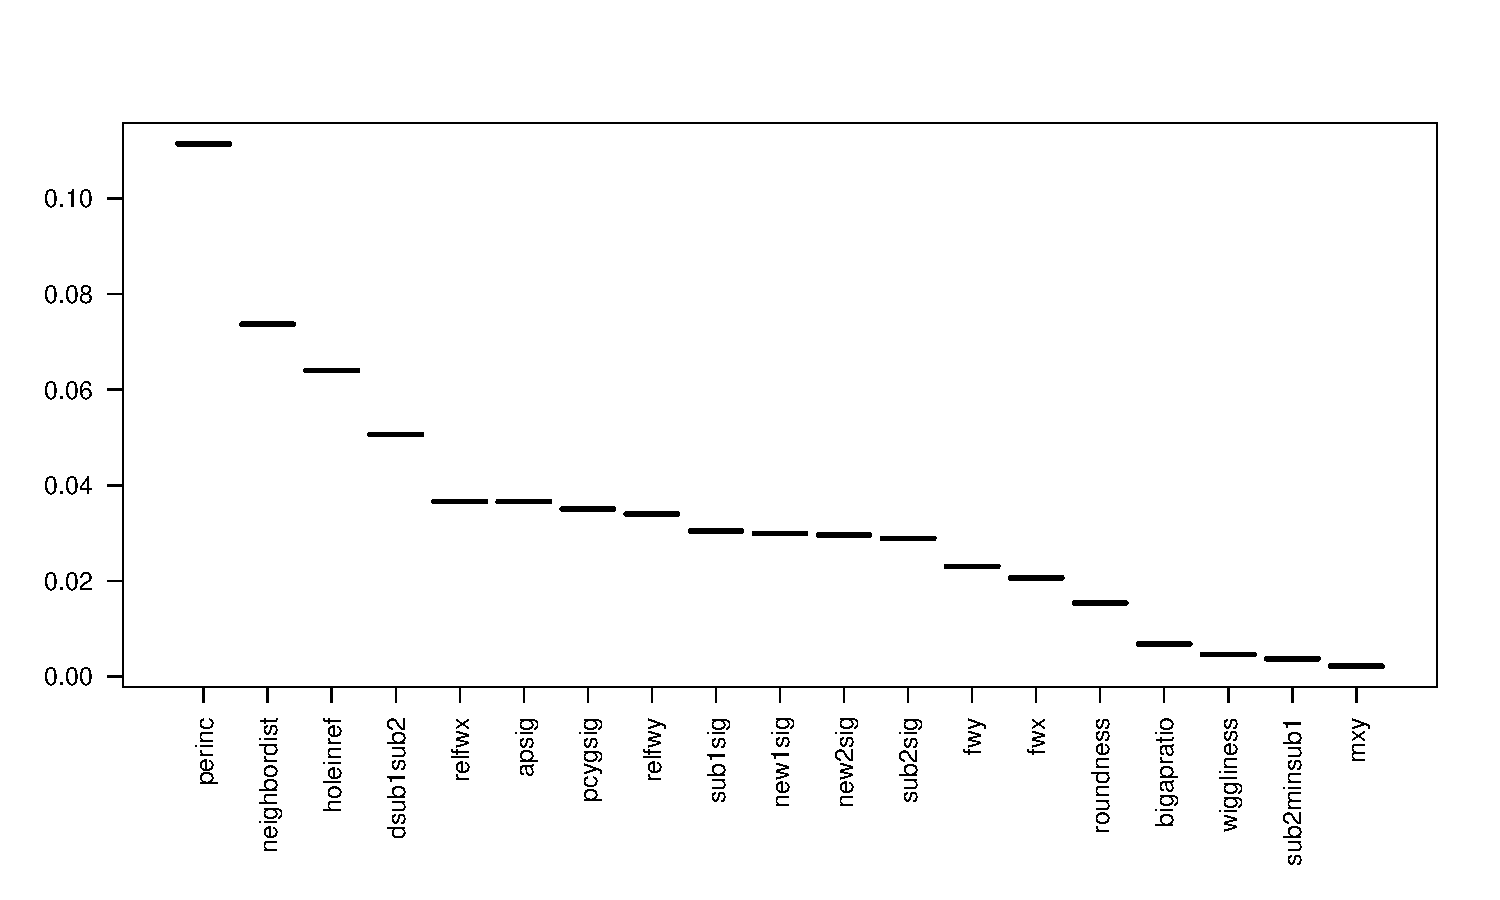
\includegraphics{imp.pdf}
\end{frame}

\begin{frame}[fragile]
	\frametitle{Supernova Data - Try different K}
	\begin{itemize}
		\item K = 2
		\begin{table}
		\begin{tabular}{cr|rr}
		& & \multicolumn{2}{c}{Prediction}\\
		& & Other & Supernova\\
		\hline
		\multirow{2}{*}{\rotatebox{90}{Actual}} & Other &  484 &  16\\
		& Supernova & 38 &  462\\
		\end{tabular}
		\end{table}
		Error: 5.4\%
		
		\item K = 8
		\begin{table}
		\begin{tabular}{cr|rr}
		& & \multicolumn{2}{c}{Prediction}\\
		& & Other & Supernova\\
		\hline
		\multirow{2}{*}{\rotatebox{90}{Actual}} & Other &  480 &  20\\
		& Supernova & 37 &  463\\
		\end{tabular}
		\end{table}
		Error: 5.7\%
	\end{itemize}
\end{frame}

\section{Boosting}
\begin{frame}
	\frametitle{Boosting}
	Idea in the binary classification context ($Y \in \{-1,1\}$).
	\begin{itemize}
		\item Take a weak classifier (one that does just a bit better than random guessing).
		\item Fit the classifier to the data to get $G_1(X)$.
		\item Give more weight to the observations in the training set it gets wrong.
		\item Re-fit the classifier to the reweighted data.
		\item Repeat M times to get a sequence of classifiers, $G_m(X)$.
		\item The predicted value of a new data point is a \textbf{weighted} sum of classifiers. 
		\[
		G(x) = \text{sign} \left( \sum_{m=1}^M{\alpha_m G_m(x)} \right)
		\]
	\end{itemize}
\end{frame}

\begin{frame}
\frametitle{AdaBoost Algorithm}
	\begin{itemize}
		\item Gives more weight to classifiers in the sequence with low training error.	
		\item Gives more weight to observations that are misclassified.  The better the classifier overall the bigger the weight on the misclassified observations.
		\item Choice of classifier is free. Often use trees with very few splits.  Stump = tree with one split.
	\end{itemize}
\end{frame}

\begin{frame}
	\frametitle{Performance on test set}
	\begin{itemize}
		\item Trees with one split (stumps)
		\begin{table}
		\begin{tabular}{cr|rr}
		& & \multicolumn{2}{c}{Prediction}\\
		& & Other & Supernova\\
		\hline
		\multirow{2}{*}{\rotatebox{90}{Actual}} & Other &  451 &  49\\
		& Supernova & 47 &  453\\
		\end{tabular}
		\end{table}
		Error: 9.6\% 
		\setkeys{Gin}{width = 0.8\textwidth}
		\begin{figure}
		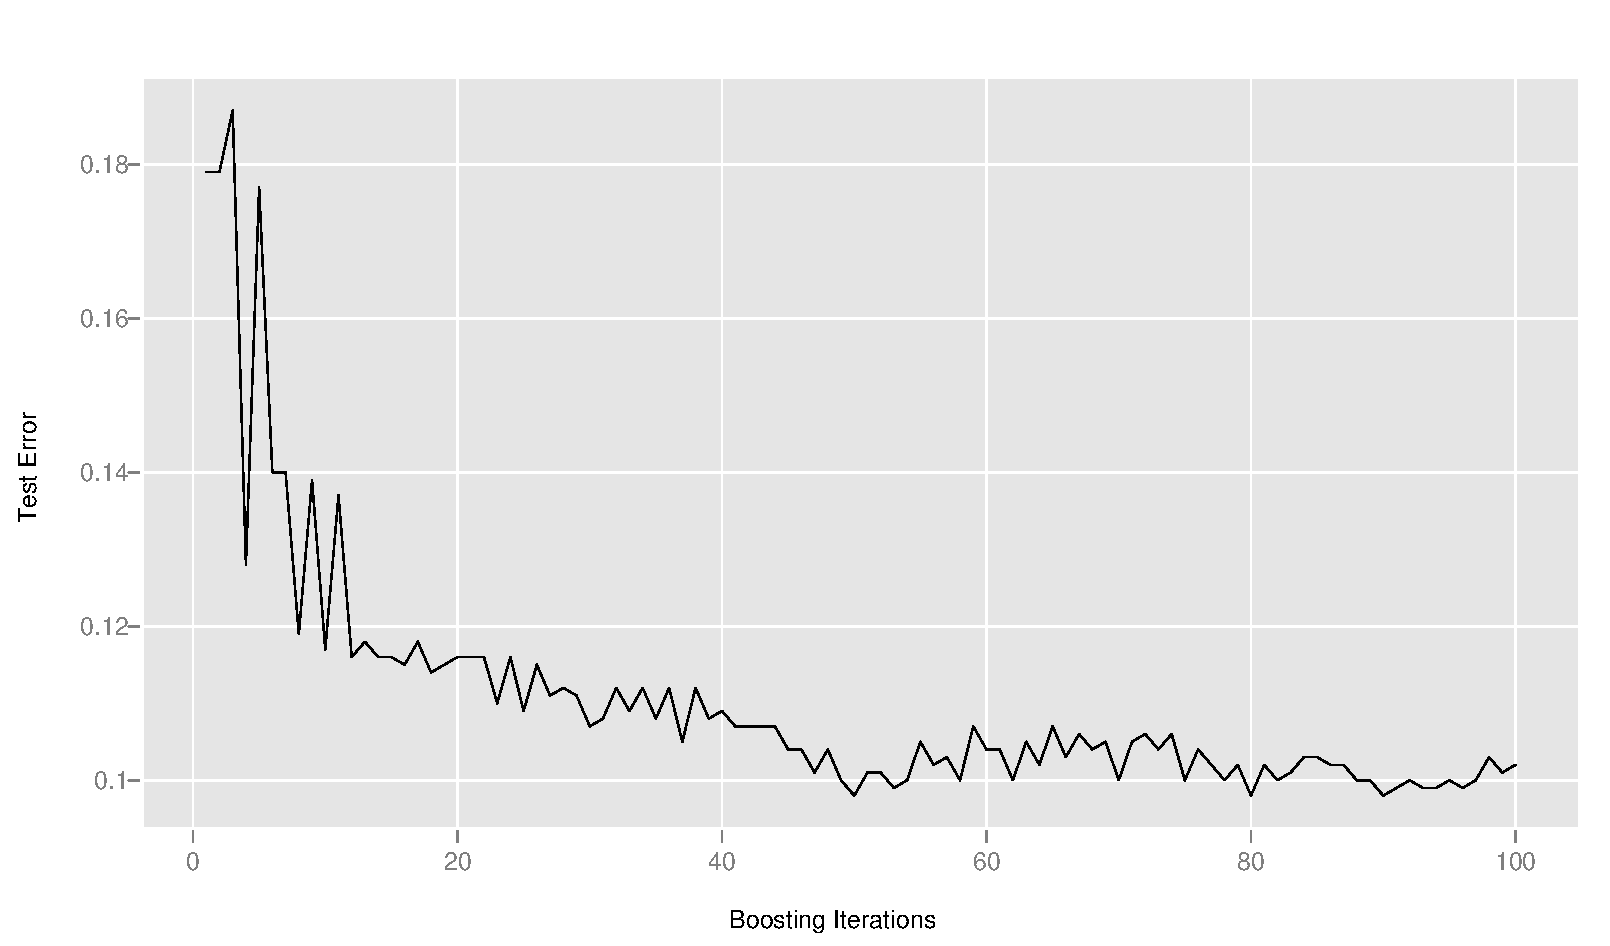
\includegraphics{error.pdf}
		\end{figure}
			\end{itemize}

\end{frame}

\begin{frame}
		Got about 8\% from CART and 6\% from bagging and 5\% from random forests.
		\begin{itemize}
			\item Trees with two splits
			\begin{table}
			\begin{tabular}{cr|rr}
			& & \multicolumn{2}{c}{Prediction}\\
			& & Other & Supernova\\
			\hline
			\multirow{2}{*}{\rotatebox{90}{Actual}} & Other &  455 &  45\\
			& Supernova & 45 &  455\\
			\end{tabular}
			\end{table}
			Error: 9.0\%
			
			\item Trees with three splits
			\begin{table}
			\begin{tabular}{cr|rr}
			& & \multicolumn{2}{c}{Prediction}\\
			& & Other & Supernova\\
			\hline
			\multirow{2}{*}{\rotatebox{90}{Actual}} & Other &  455 &  45\\
			& Supernova & 47 &  453\\
			\end{tabular}
			\end{table}
			Error: 9.2\%
		\end{itemize}
\end{frame}

\section{Neural Networks}
\begin{frame}
	\frametitle{Neural Networks}
	Simplest case
	\begin{itemize}
		\item Have p inputs $\pmb{x}$
		\item Have one hidden layer with each unit being a function ($\phi_j$) of a linear combination of the inputs. 
		\item Each output is a function ($\phi_0$) of a linear combination of the hidden units.
	\end{itemize}
	
	\begin{figure}
	\setkeys{Gin}{width = 0.6\textwidth}
	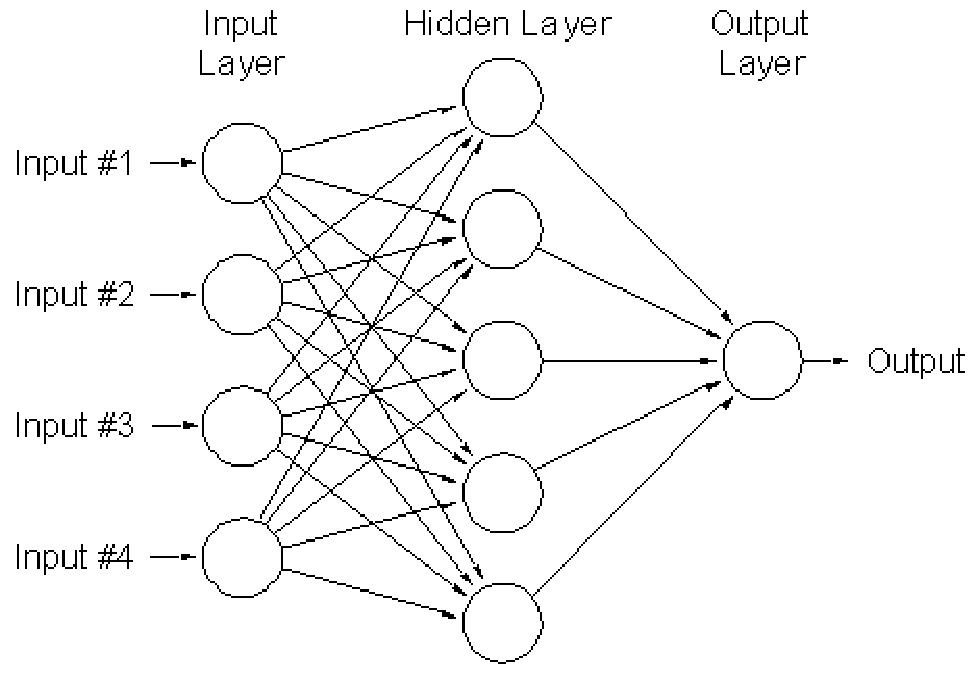
\includegraphics{nnet.pdf}
	\end{figure}
	
\end{frame}


\begin{frame}
	\frametitle{In practice}
	\begin{itemize}
		\item Scale all variables to have mean 0 variance 1 - to ensure input treated equally in regularization.
		\item Choose decay parameter by cross validation.
		\item Number of hidden units generally doesn't matter as long as it is big enough.
		\item Can be sensitive to initial conditions.  Can average a few instances.
	\end{itemize}
\end{frame}

\begin{frame}[fragile]
	\frametitle{Cross validation}
	\begin{verbatim}
		      size decay      fit
		 [1,]    5 0.010 4.333333
		 [2,]    5 0.050 4.377778
		 [3,]    5 0.001 4.600000
		 [4,]   10 0.010 4.133333
		 [5,]   10 0.050 3.977778
		 [6,]   10 0.001 4.411111
		 [7,]   15 0.010 4.366667
		 [8,]   15 0.050 4.322222
		 [9,]   15 0.001 4.388889
		[10,]   20 0.010 4.422222
		[11,]   20 0.050 4.433333
		[12,]   20 0.001 4.511111
	\end{verbatim}
	Fit neural net with 10 hidden units and decay 0.05.  Repeat five times and average result.
\end{frame}

\begin{frame}
	\frametitle{Supernova data}
	\begin{itemize}
		\item Disagreement between repetitions
			\begin{table}
			\begin{tabular}{cr|rr}
			& & \multicolumn{2}{c}{NN 1}\\
			& & Other & Supernova\\
			\hline
			\multirow{2}{*}{\rotatebox{90}{NN 2}} & Other &  495 &  15\\
			& Supernova & 10 &  480\\
			\end{tabular}
			\end{table}
			2.5\% disagreement
		\item Prediction error
			\begin{table}
			\begin{tabular}{cr|rr}
			& & \multicolumn{2}{c}{Prediction}\\
			& & Other & Supernova\\
			\hline
			\multirow{2}{*}{\rotatebox{90}{Actual}} & Other &  477 &  23\\
			& Supernova & 28 &  472\\
			\end{tabular}
			\end{table}
				5.1\% error
	\end{itemize}
\end{frame}

\begin{frame}
	\frametitle{Summary}
	Error rates:
	\begin{enumerate}

		\item 	Support vector machines $\approx$ 5\%

		\item 	Neural Networks $\approx$ 5\%

		\item 	Random Forests $\approx$ 5\%

		\item 	Bagged Trees $\approx$ 6\%

		\item 	Classification Trees $\approx$ 8\%

		\item 	Boosted Trees $\approx$ 9\%

	\end{enumerate}


\end{frame}

\begin{frame}
\end{frame}


\begin{frame}
	\begin{tiny}
	\begin{tabular}{lp{3in}}
		\hline
		Variable name & Description \\
		\hline
		apsig & signal-to-noise ratio in aperture \\
		perinc & \% flux increase in aperture from REF to NEW\\
		pcygsig & difference of flux in 2*FWHM of aperture and 0.7*FWHM; detects misaligned REF and NEW
		images)\\
		mxy & x-y moment of candidate\\
		fwx & FWHM of candidate in x\\
		fwy & FWHM of candidate in y\\
		neighbordist & distance to the nearest object in REF\\
		new1sig & signal-to-noise of candidate in NEW1\\
		new2sig & signal-to-noise of candidate in NEW2\\
		sub1sig & signal-to-noise of candidate in SUB1\\
		sub2sig & signal-to-noise of candidate in SUB2\\
		sub2minsub1 & weighted signal-to-noise difference between SUB1 and SUB2\\
		dsub1sub2 & difference in pixel coordinates between SUB1 and SUB2 (motion measurement)\\
		holeinref & measure of negative pixels on REF in region of candidate\\
		bigapratio & ratio of sum of positive pixels to sum of negative pixels within aperture\\
		relfwx & REF image FWHM in x divided by NEW image FWHM in x\\
		relfwy & REF image FWHM in y divided by NEW image FWHM in y\\
		roundness & object contour eccentricity; ratio of powers in lowest order negative and positive Fourier contour		descriptors\\
		wiggliness & object contour irregularity; power in higher order Fourier contour descriptors divided by total power\\
		\hline
	\end{tabular}
	\end{tiny}
\end{frame}

\begin{frame}
	\frametitle{Random Forests variable importance}
		\begin{itemize}
			\item Use out of bag observations and randomly permute one variable.  
			\item Run the observations down the tree and record classification.
			\item Repeat for each tree.
			\item Compare the misclassification rate with the noised up variable to the out of bag estimate without permutation.
			\item Variable Importance = percent increase in misclassification.
		\end{itemize}
\end{frame}
\end{document}
